\documentclass[preprint,12pt,authoryear]{elsarticle}
\newcommand{\citetapos}[1]{\citeauthor{#1}'s \citeyearpar{#1}}  % apostrophe's in cites
\def\linenumberfont{\normalfont\small\sffamily}
\usepackage{graphicx}
\usepackage{epstopdf}
% From link below: next two lines allow caption to fill the full figure box, and caption formats to be changed (e.g. font)
% http://tex.stackexchange.com/questions/107350/caption-below-the-figure-and-aligned-with-left-side-of-figure
% http://ctan.mackichan.com/macros/latex/contrib/caption/caption-eng.pdf
\usepackage{caption}
\captionsetup[figure]{slc=off, font=footnotesize}
\captionsetup[table]{margin={4cm, 4cm}, slc=off, font=footnotesize}


\begin{document}
\section*{\large Appendix S1: Supplementary Figures}

\begin{figure}[!ht]
       \begin{center}
      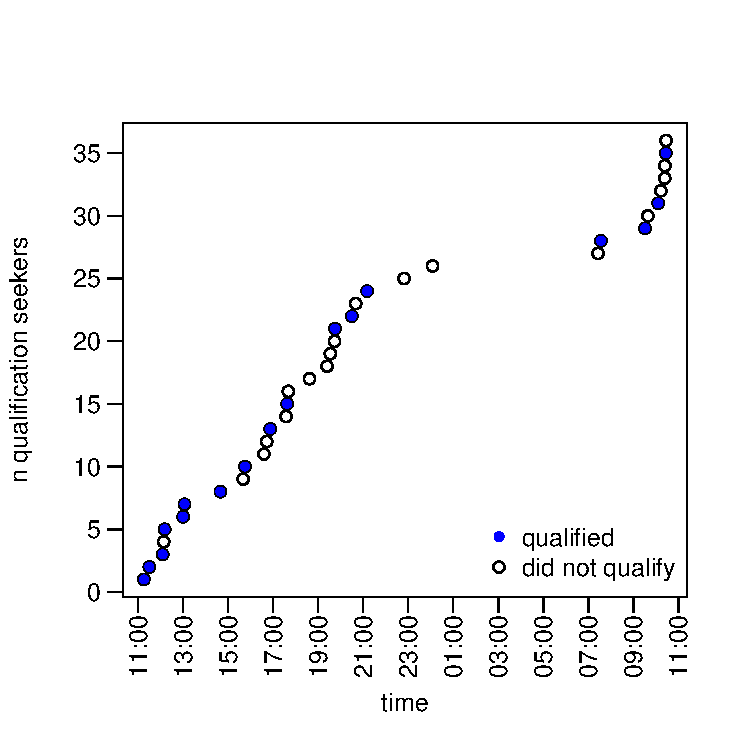
\includegraphics[scale=1]{figures/figS1.pdf} 
        \end{center}
     %\vspace{-1cm}
      \caption{The cumulative number of workers seeking qualification during the South Africa cropland mapping trial period. Successful qualification seekers are indicated by blue circles, unsuccessful by open circles.}
      \label{fig:default}
\end{figure}

\begin{figure}[!ht]
       \begin{center}
      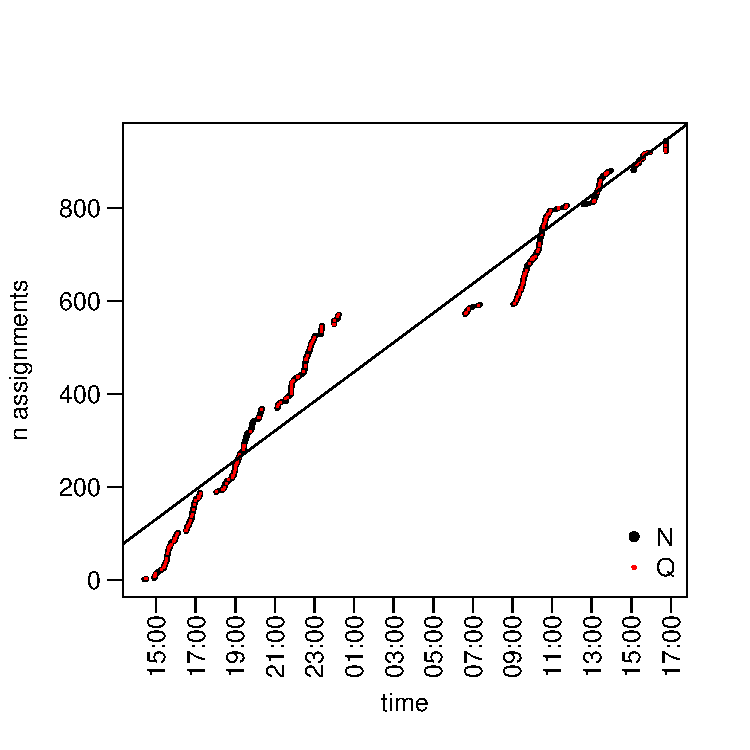
\includegraphics[scale=1]{figures/figS2.pdf} 
        \end{center}
     %\vspace{-1cm}
      \caption{The cumulative number of assignments completed during the South Africa cropland mapping trial period. Q assignments are indicated by red circles, N assignments by black circles.}
      \label{fig:default}
\end{figure}

\end{document}  

